%
% File: chap01.tex
% Author: Victor F. Brena-Medina
% Description: Introduction chapter where the biology goes.
%
\let\textcircled=\pgftextcircled
\chapter{Introduction and Motivation}
\label{chap:intro}

\initial{M}aritime travel has been a cornerstone of human civilization, facilitating the exchange of goods, ideas, and cultures across vast expanses of water. The annals of history are replete with instances of seafaring civilizations harnessing the power of wind to propel their vessels across the oceans. It is posited that ancient Neanderthals embarked on maritime voyages in the southern Ionian Islands between 110 to 35ka BP [1]. The quintessence of maritime travel has predominantly been wind-powered sails, which remained unchallenged until the industrial revolution ushered in the era of fuel-powered engines.

The art and science of sailing have evolved significantly over millennia, from rudimentary rafts and canoes to sophisticated sailing ships with complex rigging systems. Ancient civilizations, including the Egyptians, Phoenicians, and Polynesians, made remarkable advancements in sailing technology, enabling them to explore and trade over larger swathes of the ocean [2]. The medieval period saw the advent of the compass and the astrolabe, which further facilitated maritime navigation and exploration. The Age of Discovery, epitomized by the voyages of Columbus, Vasco da Gama, and Magellan, was propelled by advancements in sailing technology, which enabled transoceanic voyages and the establishment of maritime empires.

The industrial revolution in the 18th and 19th centuries marked a significant turning point in maritime propulsion. The invention of the steam engine heralded the decline of wind-powered sailing and the ascendancy of fuel-powered propulsion systems. Steamships and later, diesel-powered ships, offered greater reliability, speed, and capacity compared to their wind-powered predecessors, thus becoming the preferred mode of maritime transportation [3]. The transition to fuel-powered engines also mirrored the broader industrial and technological advancements of the era, which prioritized speed and efficiency over traditional methods.

\subsection{A Renewed Interest in Wind Propultion}
However, the environmental costs of fuel-powered maritime transportation have become increasingly apparent in the modern era. The shipping industry is a notable contributor to global carbon emissions, and the deleterious effects of pollution on marine ecosystems are well-documented [4]. These challenges have rekindled interest in wind propulsion as a sustainable alternative, prompting a re-examination of the principles that guided ancient and medieval sailors. The modern iteration of wind propulsion seeks to amalgamate the age-old wisdom of harnessing wind power with contemporary technological advancements to create eco-friendly and efficient maritime transportation systems.

Contemporary wind propulsion technologies like Flettner rotors, wing sails, and kite systems are being revisited to mitigate the environmental impact of maritime travel [3]. Among these, kite-powered vessel technology stands out due to its potential for higher efficiency and lower operational costs. Kites offer two main advantages over traditional sails: they can move relative to the vessel and can be flown at higher altitudes, accessing different wind systems.

The relative movement of kites generates apparent wind, allowing for maximum potential force even when the vessel is stationary. This enhanced apparent wind results in a larger force compared to a sail of equivalent area. Flying kites at higher altitudes taps into stronger and more consistent wind currents, making wind a more reliable energy source for propulsion [6].

However, the effective operation of kite-powered vessels requires precise control, which is skill-intensive. To leverage the full benefits of kites as a scalable propulsion method, implementing autonomous control is crucial. 

\subsection{Reinforcement Learning for Autonomous Control}
Reinforcement Learning (RL), a subset of artificial intelligence, presents a compelling avenue for optimizing the autonomous control of kite-powered vessels. The paradigm of RL, predicated on the principles of learning from interaction with the environment, holds promise for devising sophisticated control strategies that can significantly enhance the energy efficiency and operational efficacy of kite-powered vessels [4].

Talk about what we are going to investigate in the paper

% The objective of this paper is to delineate a novel Reinforcement Learning approach aimed at optimizing the autonomous control of kite-powered vessels. By leveraging the prowess of RL, we endeavor to address the challenges inherent in autonomous sail control, thereby contributing to the overarching goal of sustainable and efficient maritime transportation. The ensuing discourse will elucidate the theoretical underpinnings of our approach, the experimental setup, and the empirical findings, underscoring the potential benefits in terms of reducing operational costs and mitigating environmental impact.


\section*{Aims and Objectives}

Overall aim : Develope a RL algorithm for autonomous control of kite-powered vessels

Along the way:


% %A figures matrix.
% \begin{figure}[t!]
% \centering
% \begin{minipage}{3.3cm}
%     \centering
%     \subtop[]{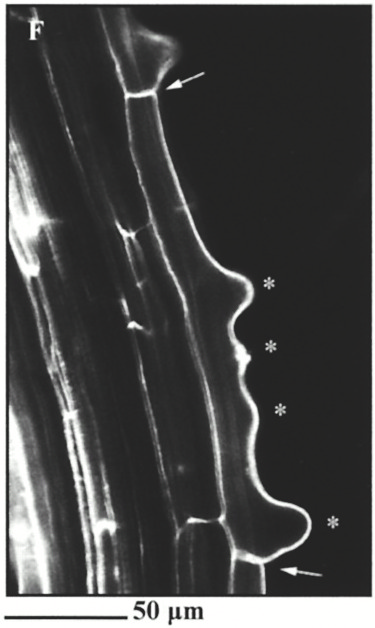
\includegraphics[height=0.28\textheight]{fig01/Nswellings}\label{sf:multiRH02a}}
% \end{minipage}
% \hspace{0.5cm}
% \begin{minipage}{3.3cm}
%     \centering
%     \subtop[]{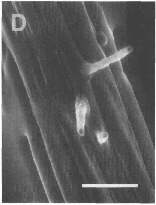
\includegraphics[height=0.27\textheight]{fig01/Mswellings}\label{sf:multiRH02b}}
% \end{minipage}
% \hspace{1.3cm}
% \begin{minipage}{3.3cm}
%     \centering
%     \subtop[]{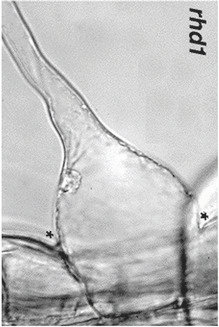
\includegraphics[height=0.27\textheight]{fig01/rhd1}\label{sf:multiRH02c}}
% \end{minipage}
% \\ \vspace{0.1cm}
% \begin{minipage}{10cm}
%     \centering
%     \subtop[]{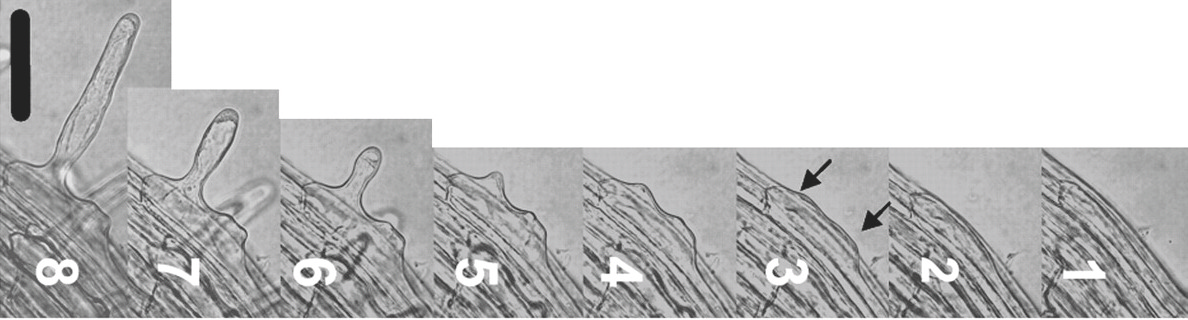
\includegraphics[height=0.145\textheight]{fig01/mutantrhd6}\label{sf:multiRH02d}}
% \end{minipage}
% \\ \vspace{0.1cm}
% \begin{minipage}{10cm}
%     \centering
%     \subtop[]{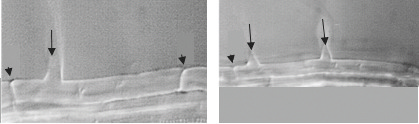
\includegraphics[height=0.16\textheight]{fig01/auxab}\label{sf:multiRH02e}}
% \end{minipage}
% \mycaption[Hair-forming mutant cells.]{(a) A mutant RH cell. Asterisks show multiple sites of RH initiation in a single root hair cell (indicated by the arrows). Figure reproduced from \cite{rigas01}. (b)~Hair-forming cell with three RH initiation locations. The bar represents $50\mu m$. Figure reproduced from \cite{massuci01}. (c) Large bump in mutant {\itshape rhd1}. Figure reproduced from \cite{griersonRH}. (d) Mutant overexpressing gene {\itshape ROP2}; from right-hand to left-hand, numbers indicate progressive snapshots at different times. RH initiation sites are indicated by the arrows. The bar represents $75\mu m$. Figure reproduced from~\cite{mjones01}. (e)~Mutants affected by auxin. On the left-hand side, RH site is farther away from the apical end (left arrow cap); on the right-hand side, multiple RH locations (arrows). Figure reproduced from~\cite{payne01}.}
% \label{fig:multiRH02}
% \end{figure}

% % A single figure
% \begin{figure}[t!]
% 	\centering
% 	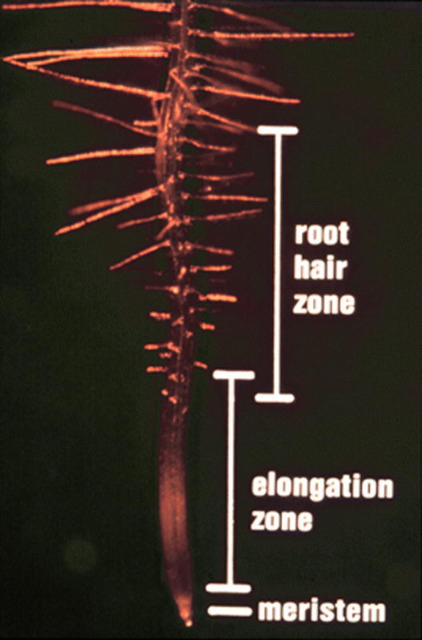
\includegraphics[height=0.35\textheight]{fig01/devepzones}
% 	\mycaption[Developmental zones of an Arabidopsis root.]{Developmental zones of an Arabidopsis root. Figure reproduced from \cite{griersonRH}.}
% 	\label{fig:RHP02}
% \end{figure}

%=========================================================